% This must be in the first 5 lines to tell arXiv to use pdfLaTeX, which is strongly recommended.
\pdfoutput=1
% In particular, the hyperref package requires pdfLaTeX in order to break URLs across lines.

\documentclass[11pt]{article}

% Remove the "review" option to generate the final version.
\usepackage[]{acl}

% Standard package includes
\usepackage{times}
\usepackage{latexsym}



% For proper rendering and hyphenation of words containing Latin characters (including in bib files)
\usepackage[T1]{fontenc}
% For Vietnamese characters
% \usepackage[T5]{fontenc}
% See https://www.latex-project.org/help/documentation/encguide.pdf for other character sets

% This assumes your files are encoded as UTF8
\usepackage[utf8]{inputenc}

% This is not strictly necessary, and may be commented out,
% but it will improve the layout of the manuscript,
% and will typically save some space.
\usepackage{microtype}

\usepackage{graphicx}
\graphicspath{ {./images/} }

% If the title and author information does not fit in the area allocated, uncomment the following
%
%\setlength\titlebox{<dim>}
%
% and set <dim> to something 5cm or larger.

\title{\\Foundations of NLP - PROJECT \\}

  \author{DANCI Laurentiu-Cristian \\
  \texttt{laurentiu-cristian.danci@s.unibuc.ro}}

\begin{document}
\maketitle
\begin{abstract}
\textbf This paper has the purpose of implementing a method to detect the irony from social media posts.
The dataset considered is the SemEval2018 Task 3 dataset including 3834 tweets classified as ironic or non-ironic.
  A machine learning application for detecting irony in social media posts can be used by authorities for predicting behaviour of social media users.
  This can help to prevent situations when bad intended people really mean the intentions that they describe in their online posts.
    Also, sometimes excessive irony about important aspects posted on social media can mean that the person suffers from anxiety or depression.
\end{abstract}

\section{Introduction}
\label{sec:intro}

The projects tries to find a method to classify texts as ironic or non-ironic.
This includes analyzing the dataset texts to extract statistics about the tweets to find out the common hashtags, emojis, tweet lengths and so on for each class.
After tokenizing the texts, the tokens are fed in a neural network that should predict the irony of the text.
The built network is a binary classifier.

\section{Related work and literature review}
\label{sec:related-work-and-literature-review}

Antonio Reyes, Paolo Rosso and Tony Veale and their paper entitled "A multidimensional approach for detecting irony in Twitter" analyze irony in terms of discriminative features that can help to automatically differentiate irony from non-irony.
Irony allows someone to express something's meaning by using words that should signify the opposite.
Their model extracts different kinds of features from texts: signatures ( counter-factuality), unexpectedness, style (it is captured by character-grams) and emotional scenarios (imagery).
In the paper "Multi-view informed attention-based model for Irony and Satire detection in Spanish variants" by Reynier Ortega-Bueno, Paolo Rosso and Jose E. Medina Pagola is mentioned that there are two main approaches to deal with the irony in texts: features-based machine learning and deep learning-based approaches.
The deep learning methods include word embeddings, Convolutional Neural Networks (CNNs) and Recurrent Neural Networks (RNNs).
The implementation in the paper is a MvAttLSTM - multi-view informed attentive LSTM\@.
LSTM or Long short term memory is a type of RNN\@.
Those multi-views include linguistics-view (stylistic, structural, semantics, affective groups of features), task-independent embedding view (encode the whole text into a single dense vectors based on deep learning models) and task-depended embedding view (pre-trained contextualized models like the ones used for sentiment analysis).
The different views are fused together by two strategies: early fusion and contextual fusion.
  Early fusion means to separately learn different features from the training data and join the representations to retain information while reducing the redundant ones.
  Contextual fusion included enriching the model with additional external knowledge to take advantage of the initial memory cell in the LTSMs layers.
  The model performs better when it is enriched with the three views.


\section{Data}\label{sec:data}

  The data includes the dataset from SemEval2018 Task 3 which is divided in three types: texts without emojis and hashtags, texts with emojis and texts with both the emojis and hashtags.
  The first step is to preprocess the data and tokenize each word in a token.
  For this task, a customized preprocessor was written.
  This preprocessor does the following tasks: (1) converts the casing to lower case, (2) converts emoticons (example: ":)", ":D") to emojis (unicode characters), (3) translate emojis to text description (for example "sad face"), (4) handles hashtags - remove the \# symbol (so the hashtags are usual words) or remove the words entirely and keep them as they already are (this can be used to give another meaning to the hashtag when creating the word vectors), (5) removes numbers, (6) removes punctuation and (7) convert slang to usual words (for example: convert IRL to in real life).
Analyzing the datasets yields the following information about the most common hashtags, emojis presented in the following graphs.

\begin{figure}[h!]
  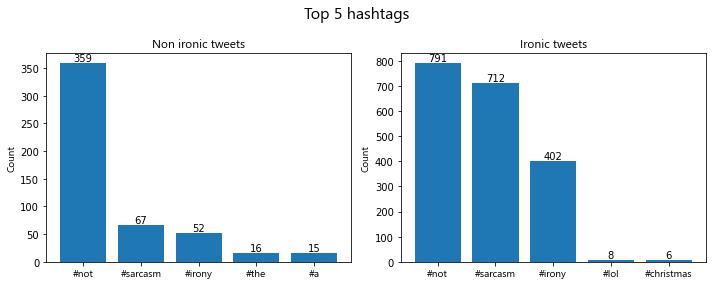
\includegraphics[width=\columnwidth]{hashtags}
  \caption{Hashtags distributed among non-ironic and ironic tweets}\label{fig:figure9}
\end{figure}

\begin{figure}[h!]
  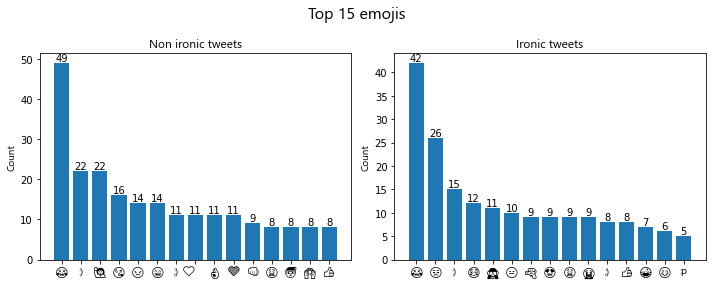
\includegraphics[width=\columnwidth]{emojis}
  \caption{Most common emojis}\label{fig:figure15}
\end{figure}

\begin{figure}[h!]
  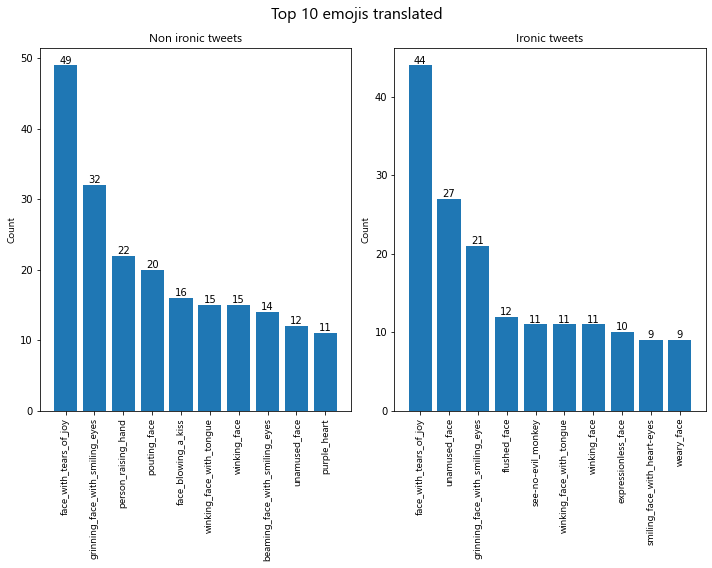
\includegraphics[width=\columnwidth]{emojis2}
  \caption{Most common emojis translated to text}\label{fig:figure14}
\end{figure}


\begin{figure}[h!]
    \begin{center}
  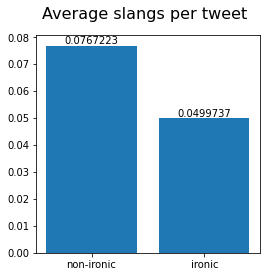
\includegraphics[scale=0.5]{slang}
  \caption{Average slang used per tweet}\label{fig:figure13}
        \end{center}
\end{figure}


  Slang words does not add meaningful information because too few tweets include slang - this can be not true, though, because it is hard to prepare a list of all internet slang words, but in this case even the most common slang are not that common.
  The ironic tweets usually contain the \#not hashtag.
  This can be because irony means the opposite of the said sentence and adding a \#not hashtag can show that.
  There are no other common tags in the dataset besides \#not, \#sarcasm and \#irony.
Looking at the SemEval website ([3]) the dataset was constructed by searching Twitter for the hashtags \#irony, \#sarcasm and \#not so it was expected to top rank those three hashtags.
  The most emojis are common in both tweet types.

  Looking at the average tokens per tweet and average number of characters per tweets, an observation is that those numbers does not have an influence on the category.


\begin{figure}[h!]
\begin{center}
  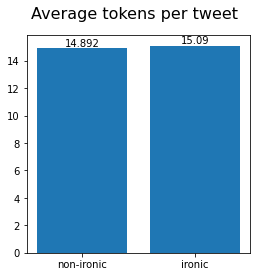
\includegraphics[scale=0.5]{avg_tokens}

  \caption{Average number of tokens}\label{fig:figure12}
      \end{center}
\end{figure}



\begin{figure}[h!]
    \begin{center}
  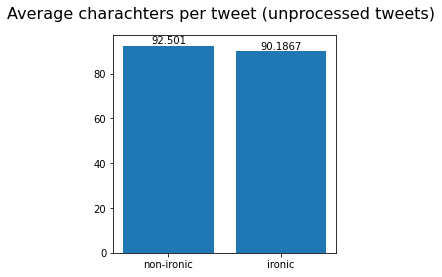
\includegraphics[width=\columnwidth]{avg_chars}

  \caption{Average number of characters}\label{fig:figure11}
        \end{center}
\end{figure}



  As an early observation, keeping the hashtags with the \# symbol while training the model can make the network biased to give an "ironic" label tweets based only on the hashtags.
If the tokens include the \# sign, those tokens will be embedded in different vectors than the ones without the sign, so their meaning will be a different one and the correlation between the hashtags and the label would be too tight.
  This can be mitigated by removing the \# symbols or remove the hashtags altogether - this way the model can learn the other features that can give an "ironic" status to a text.
An observation is that the ironic tweets are very alike to the non-ironic tweets - this means that the irony really states in the hidden meaning of the text (the intention to mean the opposite).

  \section{Method}\label{sec:method}
The neural network functions and classes are imported from the Pytorch package.
  The machine learning method includes an embedding layer that converts the words to vectors, Long Short term memory layer that can process a sequence of data (the sequence of tokens that make a sentence) and a fully connected (linear) layer that has only one output that is sent through a sigmoid activation function.
  This way, the output can be rounded to the nearest integer to find out the label (0 for non-ironic and 1 for ironic).
  This is a binary classifier.
  The loss function is BCELoss that is used for binary classifiers, and the optimizer is an Adam optimizer.
For the word embeddings, the size of the vectors is 100 and the hidden.
The hidden dimension size for the Long Short Term Memory layer is half of the embedding dimension.
Those arbitrary chosen dimensions can be changed running a parameter grid search if the initial results are not satisfactory, but the main idea of the project is to check out if the overall arhitecture of the application would work.

\begin{figure}[h!]
      \begin{center}
  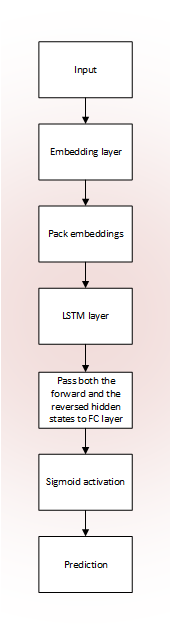
\includegraphics[scale=0.8]{nn}
  \caption{Neural network arhitecture and flow}\label{fig:figure10}
          \end{center}
\end{figure}


  Because not all tweets have the same lengths, it is needed to use the pack\_padded\_sequence function from pytorch to pad the sentences to the same length.
The LSTM layer has the parameter "bidirectional" set to "True", so the layer generates both the forward and reversed hidden states which can help with the model performance.
  A dictionary from all the tokens from the training data will be used to build an encoder that gives each token an index.
This is a required step for the embedding layer.
While testing, the unseen tokens will be replaced with an "unknown" token.

  \section{Results}\label{sec:results}

For training the model, in the preprocessing step, Twitter mentions and URLs were replaced by placeholders.
The emojis were replaced with textual descriptions, and the internet slang words replaced by their translations.
The numbers were removed altogether.
A lemmatizer was also used.
The stopwords were not removed because the meaning of the sentence could be affected - for example "not" is considered a stopword by the NLTK stopword module and negation is an important aspect of ironic tweets.

The model was trained for 20 epochs and 5-fold cross validated.
For model selection, only the models with the best validation scores are kept.
Observation: the model got over-fitted on the training data (the accuracy on training data increased, but on the validation data it decreased).
To fix this issue, a dropout of 0.5 probability was added after the LSTM.
Also, an optimizer like SGD can help the algorithm to generalize better, but converges slower, so the current Adam optimizer was configured with a weight decay of 0.001 to help with regularization.
The model over-fitting on the training data is reduced a bit.
\begin{figure}[h!]
  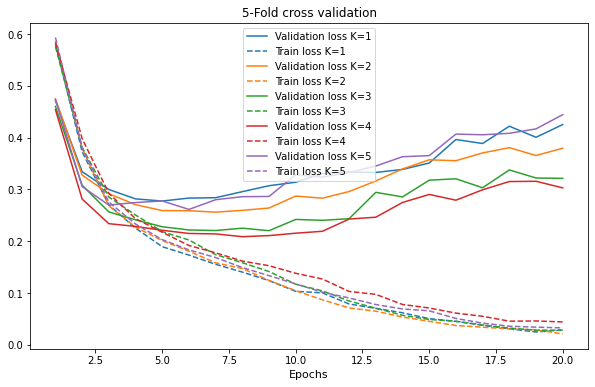
\includegraphics[width=\columnwidth]{train_loss_hashtags}
  \caption{Training and validation loss}\label{fig:figure}
\end{figure}
\begin{figure}[h!]
  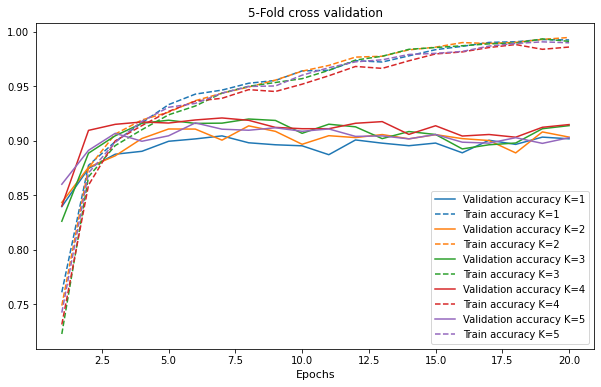
\includegraphics[width=\columnwidth]{train_acc_hashtags}
  \caption{Training and validation accuracy}\label{fig:figure2}
\end{figure}

  \begin{center}
\begin{tabular}{||c c c||}
 \hline
 K & Best val loss & Best val acc \\ [0.5ex]
 \hline\hline
 1 & 0.2776 & 0.9044 \\
 \hline
 2 & 0.2562 & 0.9136 \\
 \hline
 3 & 0.2204 & 0.9199 \\
 \hline
 4 & 0.2088 & 0.9208 \\
 \hline
 5 & 0.2614 & 0.9163 \\ [1ex]
 \hline
\end{tabular}
%      \caption{Validation results}
\end{center}

    A second model uses pretrained word embeddings.
    Gensim has a module for accessing pretrained model.
    The chosen model is "glove-twitter-100" which contain word vectors of size 100.
    The word vectors of the pretrained model replaced the weights of the embedding layer.
    The layer was frozen so in the training stage only the fully connected layer is trainable.

\begin{figure}[h!]
  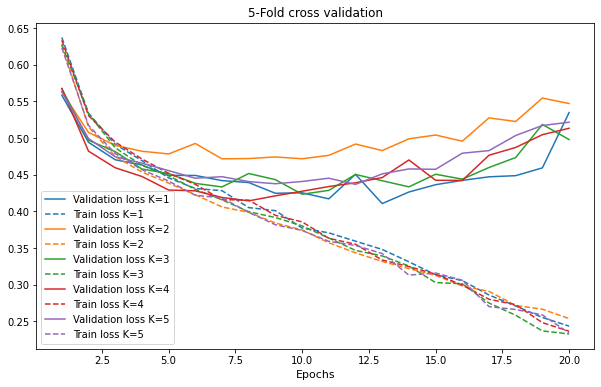
\includegraphics[width=\columnwidth]{train_loss_hashtags_pretrained}
  \caption{Training and validation loss (pretrained embeddings)}\label{fig:figure4}
\end{figure}

\begin{figure}[h!]
  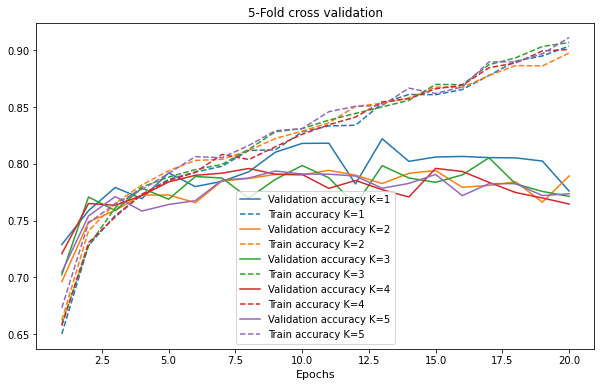
\includegraphics[width=\columnwidth]{train_acc_hashtags_pretrained}
  \caption{Training and validation accuracy (pretrained embeddings)}\label{fig:figure3}
\end{figure}

\begin{center}
\begin{tabular}{||c c c||}
 \hline
 K & Best val loss & Best val acc\\ [0.5ex]
 \hline\hline
 1 & 0.4107 & 0.8220 \\
 \hline
 2 & 0.4717 & 0.7942 \\
 \hline
 3 & 0.4234 & 0.8053 \\
 \hline
 4 & 0.4144 & 0.7959 \\
 \hline
 5 & 0.4368 & 0.7936 \\ [1ex]
 \hline
\end{tabular}
\end{center}

As we can see, the results are good for the non-pretrained embeddings - over 90\% accuracy.
But, I think that the irony hashtags had an effect far too great on the results.
For the next runs, the hashtags \#not, \#irony and \#sarcasm were removed.
In the case of the other hashtags, they were kept, including the \# symbol.

\begin{figure}[h!]
  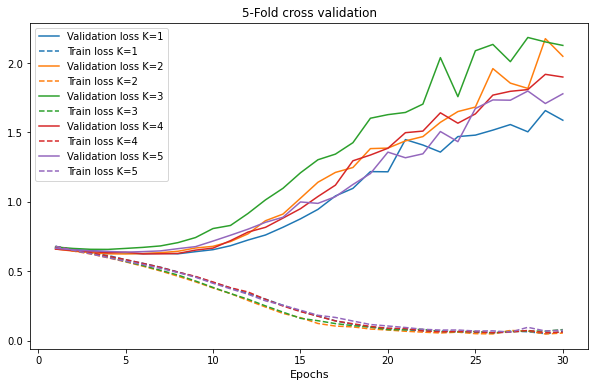
\includegraphics[width=\columnwidth]{train_loss}
  \caption{Training and validation loss (no irony hashtags)}\label{fig:figure5}
\end{figure}

\begin{figure}[h!]
  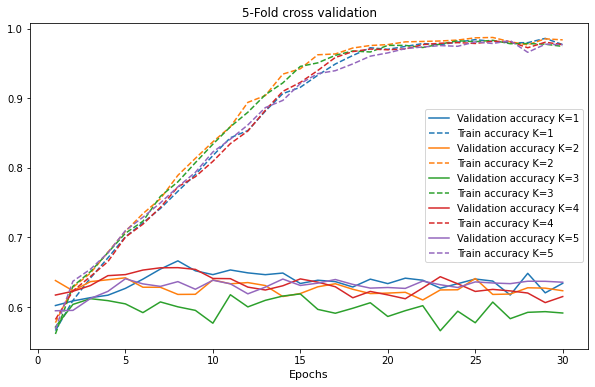
\includegraphics[width=\columnwidth]{train_acc}
  \caption{Training and validation accuracy (no irony hashtags)}\label{fig:figure6}
\end{figure}

\begin{center}
\begin{tabular}{||c c c||}
 \hline
 K & Best val loss & Best val acc\\ [0.5ex]
 \hline\hline
 1 & 0.4107 & 0.8220 \\
 \hline
 2 & 0.4717 & 0.7942 \\
 \hline
 3 & 0.4234 & 0.8053 \\
 \hline
 4 & 0.4144 & 0.7959 \\
 \hline
 5 & 0.4368 & 0.7936 \\ [1ex]
 \hline
\end{tabular}
\end{center}

\begin{figure}[h!]
  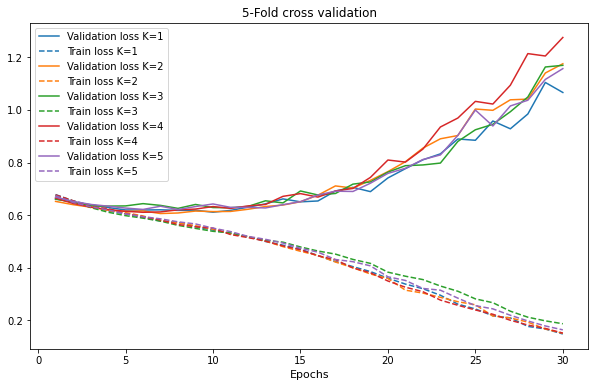
\includegraphics[width=\columnwidth]{train_loss_pretrained}
  \caption{Training and validation loss (no irony hashtags, pretrained embeddings)}\label{fig:figure7}
\end{figure}

\begin{figure}[h!]
  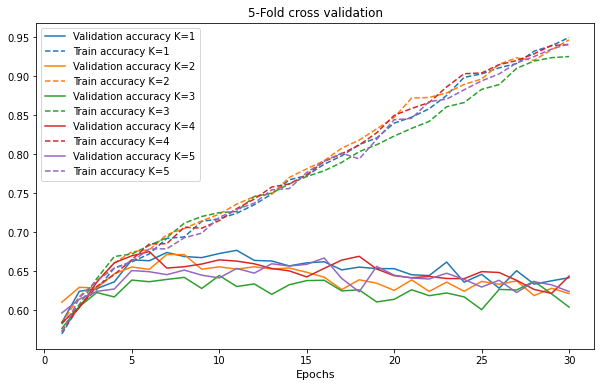
\includegraphics[width=\columnwidth]{train_accuracy_pretrained}
  \caption{Training and validation accuracy (no irony hashtags, pretrained embeddings)}\label{fig:figure8}
\end{figure}


\begin{center}
\begin{tabular}{||c c c||}
 \hline
 K & Best val loss & Best val acc\\ [0.5ex]
 \hline\hline
 1 & 0.4107 & 0.8220 \\
 \hline
 2 & 0.4717 & 0.7942 \\
 \hline
 3 & 0.4234 & 0.8053 \\
 \hline
 4 & 0.4144 & 0.7959 \\
 \hline
 5 & 0.4368 & 0.7936 \\ [1ex]
 \hline
\end{tabular}
\end{center}

    As we can see, the model gets over-fitted very fast on the training data and the validation loss increases after several epochs.

    The final results (testing the model on the test data - test data does not include the irony tags) are presented in the table.

  \begin{center}
\begin{tabular}{||c c c||}
 \hline
 Pretrained emb & Irony hashtags \# & Test acc \\ [0.5ex]
 \hline\hline
 No & Yes & 0.9218 \\
 \hline
 Yes & Yes & 0.7596 \\
 \hline
 No & No & 0.6517 \\
 \hline
 Yes & No & 0.6261 \\
 \hline
  & Random chance & 0.5213 \\
 \hline
\end{tabular}
\end{center}

    \section{Conclusions and future work}\label{sec:conclusions-and-future-work}
The model gets over-fitted on the training data which means that the network needs improvements to increase the generalisation.
A reason can be that the irony comes in many flavours, and a small dataset is not enough for catching all the characteristics of irony.
The network learns the irony in the test data, but it can not predict the irony of unseen data, as shown by the validation step and the final test.
For a real life scenario it needs a larger dataset.
Training the model with tweets including the irony hashtags yield good results on validation set, but it does not have any application outside of detecting irony in tweets already marked with the \#irony or \#not hashtags.
    Also, other features could be appended to the network to improve the performance.
    This means knowledge of linguistic concepts to engineer reliable features.
Using only embedding does not yield good results.
The accuracy is just over the random chance.

    \section{References}\label{sec:references}
    [1] "A multidimensional approach for detecting irony in Twitter" - Antonio Reyes, Paolo Rosso, Tony Veale
\newline
    [2] "Multi-view informed attention-based model for Irony and Satire detection in Spanish variants" - Reynier Ortega-Bueno, Paolo Rosso,  Jose E. Medina Pagola
\newline
    [3] https://competitions.codalab.org/competitions/17468\#learn\_the\_details-data-annotation
    \newline
    [4] https://towardsdatascience.com/how-to-preprocess-social-media-data-and-text-messages-b011efacf74
    \newline
    [5] https://pytorch.org/tutorials/beginner/nlp/sequence\_models\_tutorial.html
    \newline
    [6] https://www.analyticsvidhya.com/blog/2020/01/first-text-classification-in-pytorch/
\end{document}
